\chapter{Optimizers}



\section{Stochastic gradient descent with mini-batches}

\begin{description}
    \item[Stochastic gradient descent (SGD)] \marginnote{SGD}
        Gradient descent based on a noisy approximation of the gradient computed on mini-batches of $B$ data samples.

        An epoch $e$ of SGD with mini-batches of size $B$ does the following:
        \begin{enumerate}
            \item Shuffle the training data $\matr{D}^\text{train}$.
            \item For $u = 0, \dots, U$, with $U = \lceil \frac{N}{B} \rceil$:
            \begin{enumerate}
                \item Classify the examples $\matr{X}^{(u)} = \{ \vec{x}^{(Bu)}, \dots, \vec{x}^{(B(u+1)-1)} \}$ 
                    to obtain the predictions $\hat{Y}^{(u)} = f(\vec{X}^{(u)}; \matr{\theta}^{(e*U+u)})$
                    and the loss $\mathcal{L}\big( \matr{\theta}^{(e*U+u)}, (\matr{X}^{(u)}, \hat{Y}^{(u)}) \big)$.
                \item Compute the gradient $\nabla \mathcal{L} = \frac{\partial\mathcal{L}}{\partial \matr{\theta}}\big( \matr{\theta}^{(e*U+u)}, (\matr{X}^{(u)}, \hat{Y}^{(u)}) \big)$.
                \item Update the parameters $\matr{\theta}^{(e*U+u+1)} = \matr{\theta}^{(e*U+u)} - \texttt{lr} \cdot \nabla \mathcal{L}$.
            \end{enumerate}
        \end{enumerate}
\end{description}

\begin{remark}[Spheres] \marginnote{SGD spheres}
    GD/SGD works better on convex functions (e.g., paraboloids) as there are no preferred directions to reach a minimum. Moreover, faster convergence can be obtained by using a higher learning rate.

    \begin{figure}[H]
        \centering
        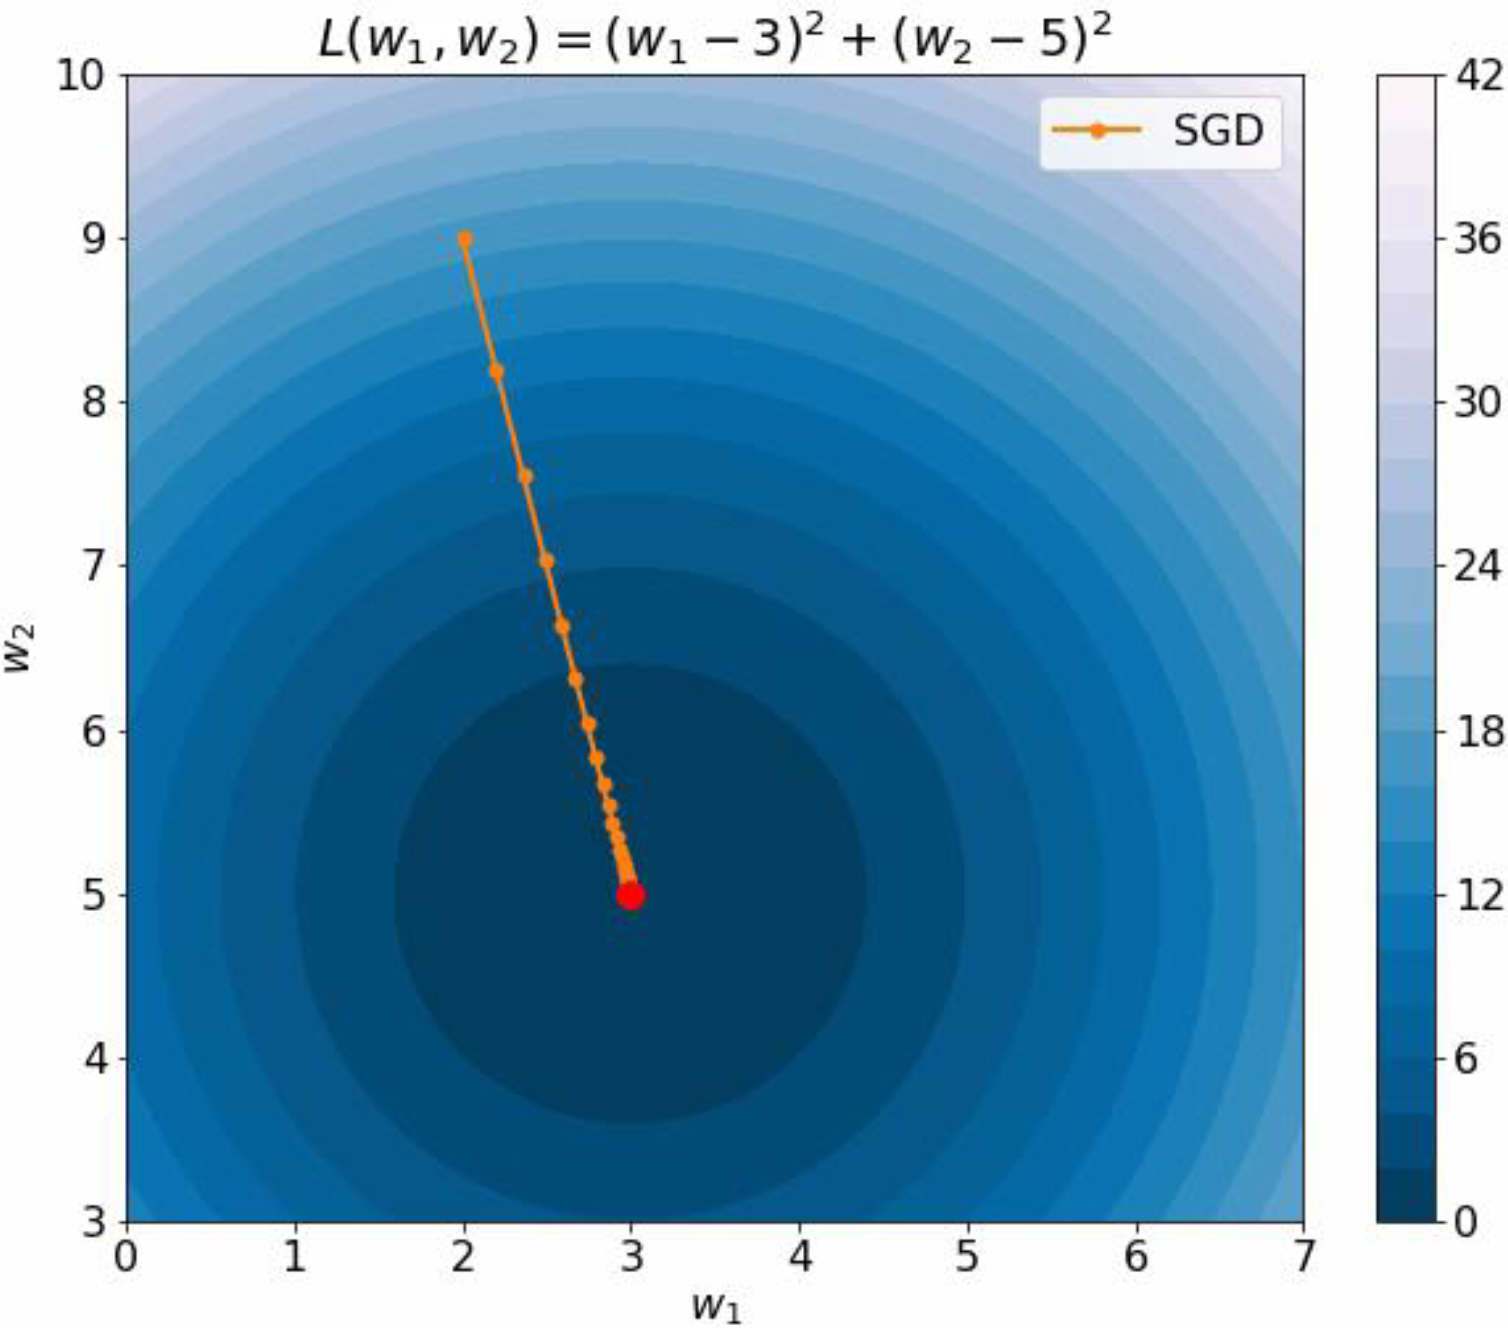
\includegraphics[width=0.35\linewidth]{./img/sgd_sphere.png}
    \end{figure}
\end{remark}

\begin{remark}[Canyons] \marginnote{SGD canyons}
    A function has a canyon shape if it grows faster in some directions.

    The trajectory of SGD oscillates in a canyon (the steep area) and a smaller learning rate is required to reach convergence. Note that, even though there are oscillations, the loss alone decreases and is unable to show the oscillating behavior.

    \begin{figure}[H]
        \centering
        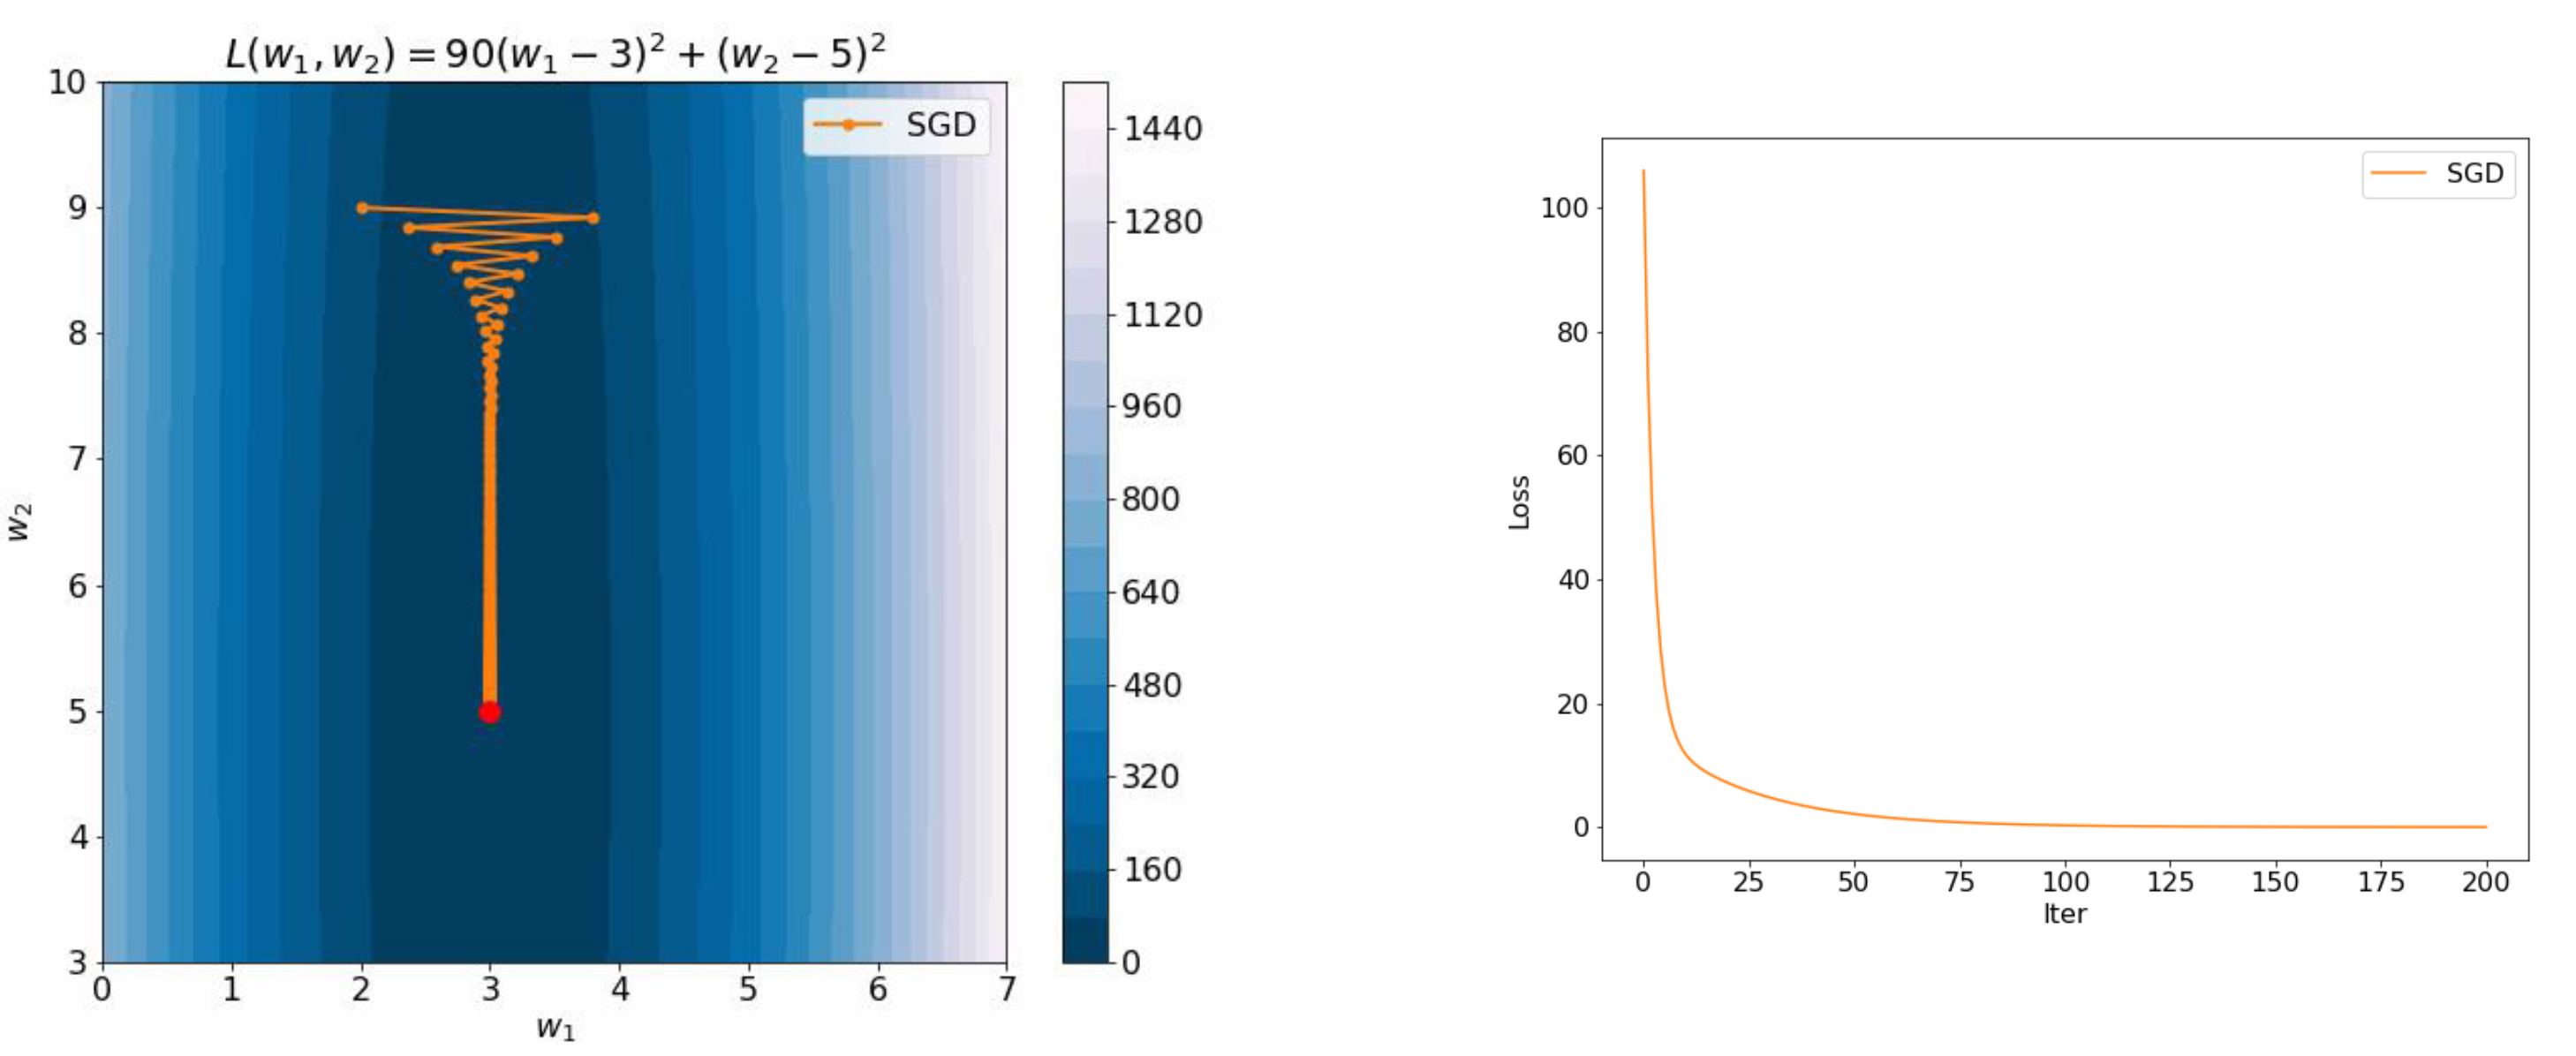
\includegraphics[width=0.8\linewidth]{./img/sgd_canyon.png}
    \end{figure}
\end{remark}

\begin{remark}[Local minima] \marginnote{SGD local minima}
    GD/SGD converges to a critical point. Therefore, it might end up in a saddle point or local minima.

    \begin{figure}[H]
        \centering
        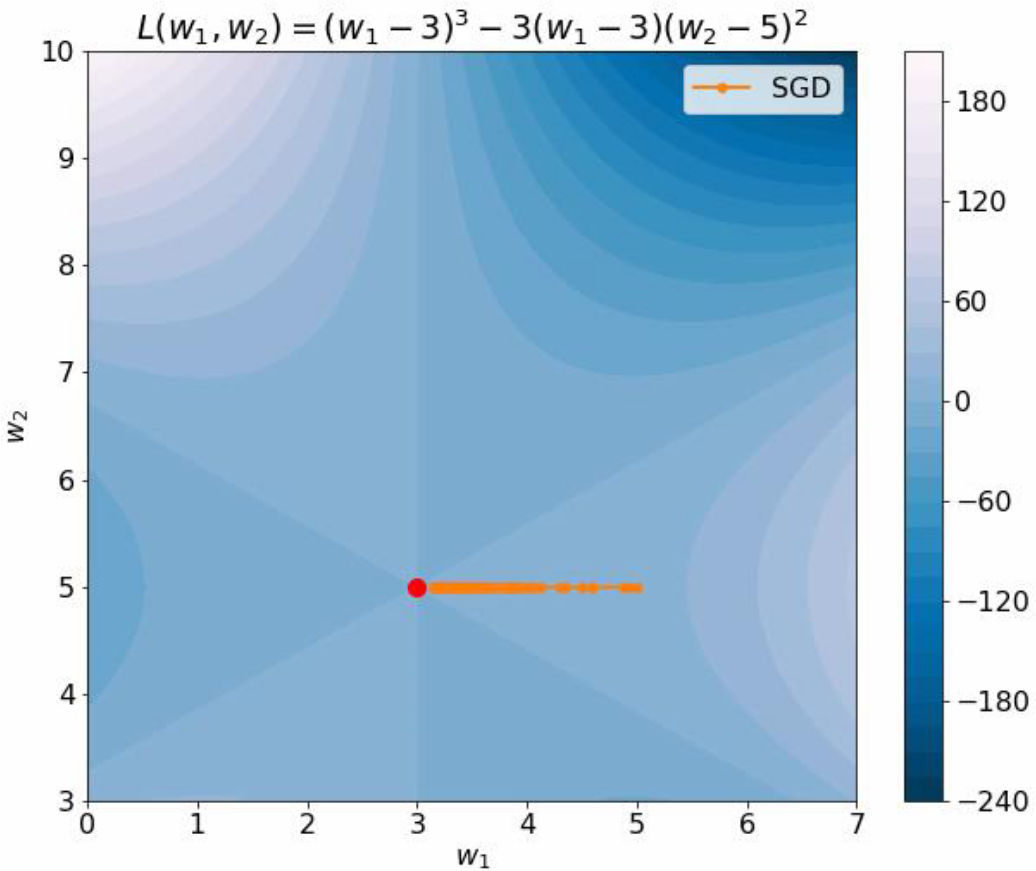
\includegraphics[width=0.35\linewidth]{./img/sgd_local_minima.png}
    \end{figure}
\end{remark}



\section{Second-order methods}

Methods that also consider the second-order derivatives when determining the step.

\begin{description}
    \item[Newton's method] \marginnote{Newton's method}
        Second-order method for the 1D case based on the Taylor expansion:
        \[ f(x_t + \Delta x) \approx f(x_t) + f'(x_t)\Delta x + \frac{1}{2}f''(x_t)\Delta x^2 \]
        which can be seen as a paraboloid over the variable $\Delta x$.

        Given a function $f$ and a point $x_t$, the method fits a paraboloid at $x_t$ with the same slope and curvature at $f(x_t)$. The update is determined as the step required to reach the minimum of the paraboloid from $x_t$. It can be shown that this step is $-\frac{f'(x_t)}{f''(x_t)}$.

        \begin{figure}[H]
            \centering
            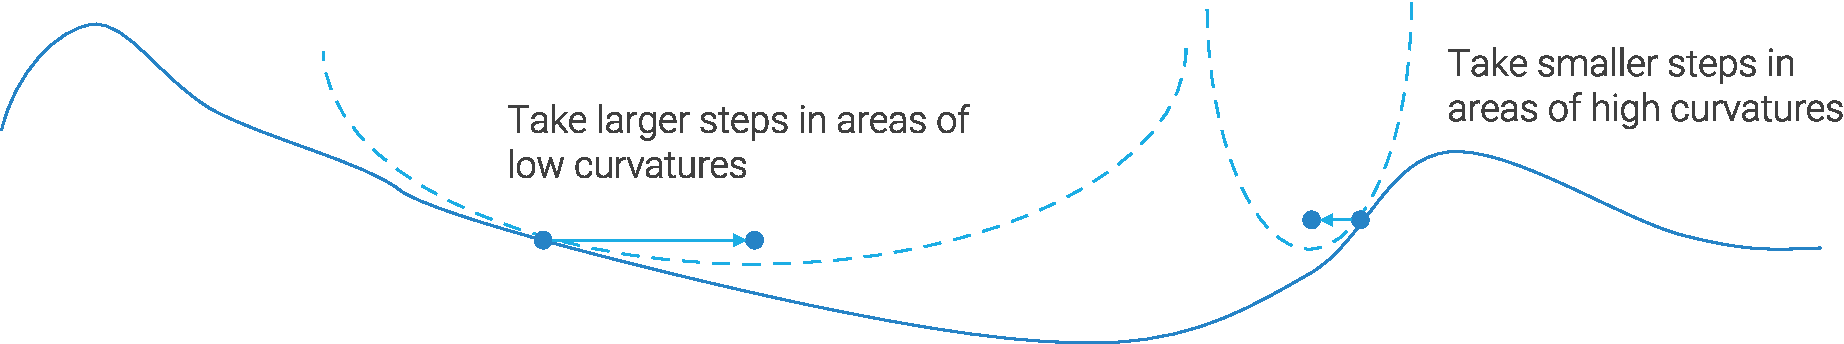
\includegraphics[width=0.7\linewidth]{./img/_2order_optimizer.pdf}
        \end{figure}
\end{description}

\begin{remark}
    For quadratic functions, second-order methods converge in one step.
    \begin{figure}[H]
        \centering
        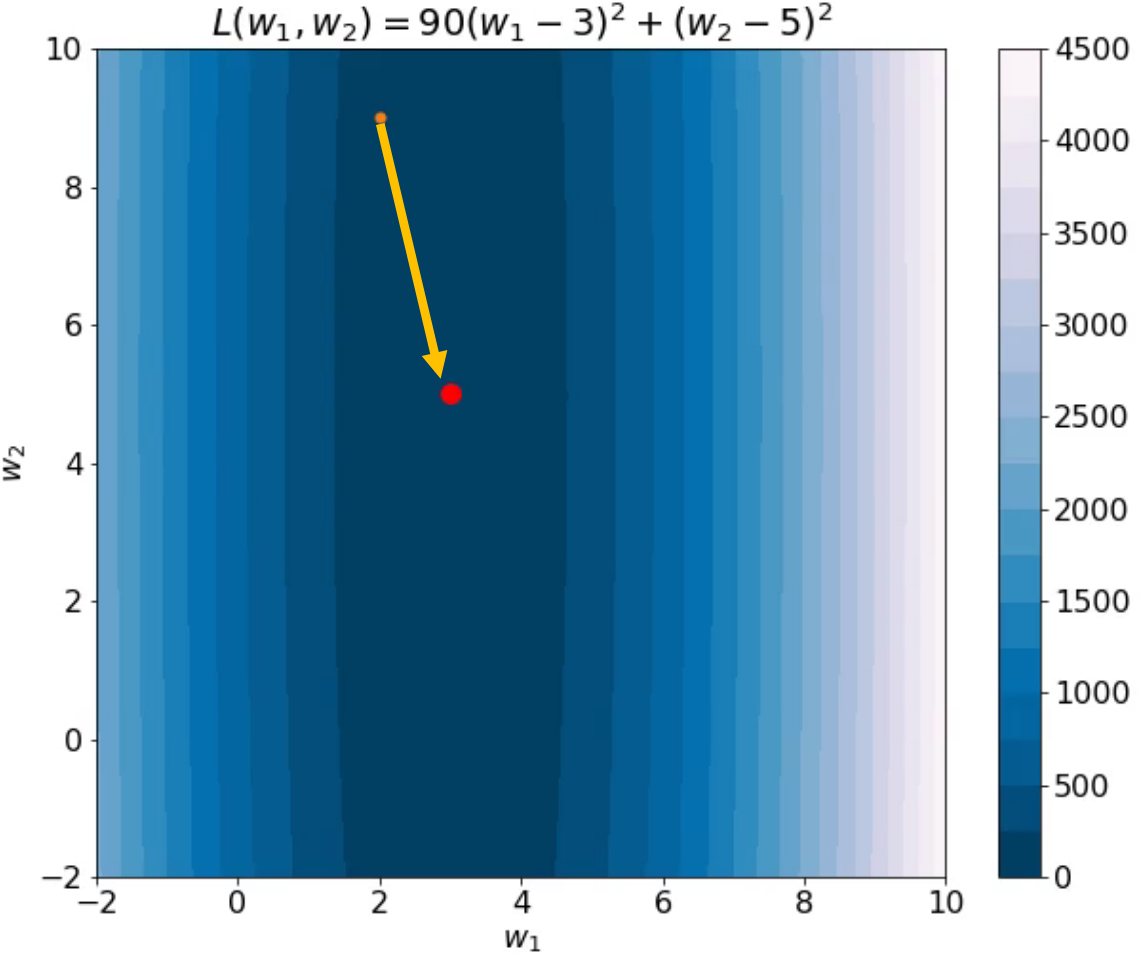
\includegraphics[width=0.35\linewidth]{./img/2order_1step.png}
    \end{figure}
\end{remark}

\begin{description}
    \item[General second-order method] \marginnote{General second-order method}
        For a generic multivariate non-quadratic function, the update is:
        \[ -\texttt{lr} \cdot \matr{H}_f^{-1}(\vec{x}_t) \nabla f(\vec{x}_t) \]
        where $\matr{H}_f$ is the Hessian matrix.

        \begin{remark}
            Given $k$ variables, $\matr{H}$ requires $O(k^2)$ memory. Moreover, inverting a matrix has time complexity $O(k^3)$. Therefore, in practice second-order methods are not applicable for large models.
        \end{remark}
\end{description}



\section{Momentum}

\begin{description}
    \item[Standard momentum]\marginnote{Standard momentum}
        Add a velocity term $v^{(t)}$ to account for past gradient updates:
        \[
            \begin{split}
                v^{(t+1)} &= \mu v^{(t)} - \texttt{lr} \nabla \mathcal{L}(\matr{\theta}^{(t)}) \\
                \matr{\theta}^{(t+1)} &= \matr{\theta}^{(t)} + v^{(t+1)}
            \end{split}
        \]
        where $\mu \in [0, 1[$ is the momentum coefficient.

        In other words, $v^{(t+1)}$ represents a weighted average of the updates steps done up until time $t$.

        \begin{remark}
            Momentum helps to counteract a poor conditioning of the Hessian matrix when working with canyons.
        \end{remark}
        \begin{remark}
            Momentum helps to reduce the effect of variance of the approximated gradients (i.e., acts as a low-pass filter).
        \end{remark}

        \begin{figure}[H]
            \centering
            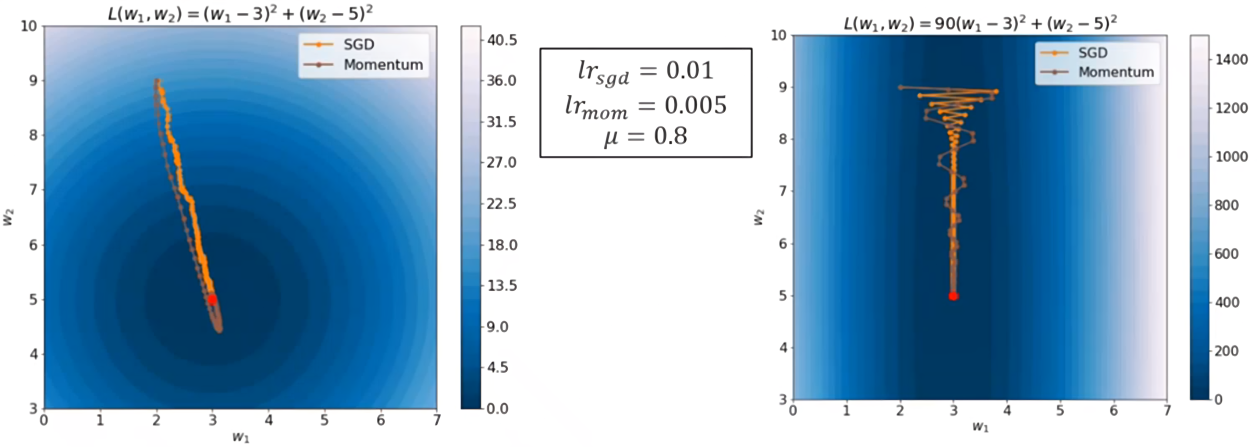
\includegraphics[width=0.8\linewidth]{./img/momentum.png}
            \caption{
                \parbox[t]{0.7\linewidth}{
                    Plain SGD vs momentum SGD in a sphere and a canyon. In both cases, momentum converges before SGD.
                }
            }
        \end{figure}

    \item[Nesterov momentum] \marginnote{Nesterov momentum}
        Variation of the standard momentum that computes the gradient step considering the velocity term:
        \[
            \begin{split}
                v^{(t+1)} &= \mu v^{(t)} - \texttt{lr} \nabla \mathcal{L}(\matr{\theta}^{(t)} + \mu v^{(t)}) \\
                \matr{\theta}^{(t+1)} &= \matr{\theta}^{(t)} + v^{(t+1)}
            \end{split}
        \]

        \begin{remark}
            The key idea is that, once $\mu v^{(t)}$ is summed to $\matr{\theta}^{(t)}$, the gradient computed at $\matr{\theta}^{(t)}$ is obsolete as $\matr{\theta}^{(t)}$ has been partially updated.
        \end{remark}

        \begin{remark}
            In practice, there are methods to formulate Nesterov momentum without the need of computing the gradient at $\matr{\theta}^{(t)} + \mu v^{(t)}$.
        \end{remark}

        \begin{figure}[H]
            \centering
            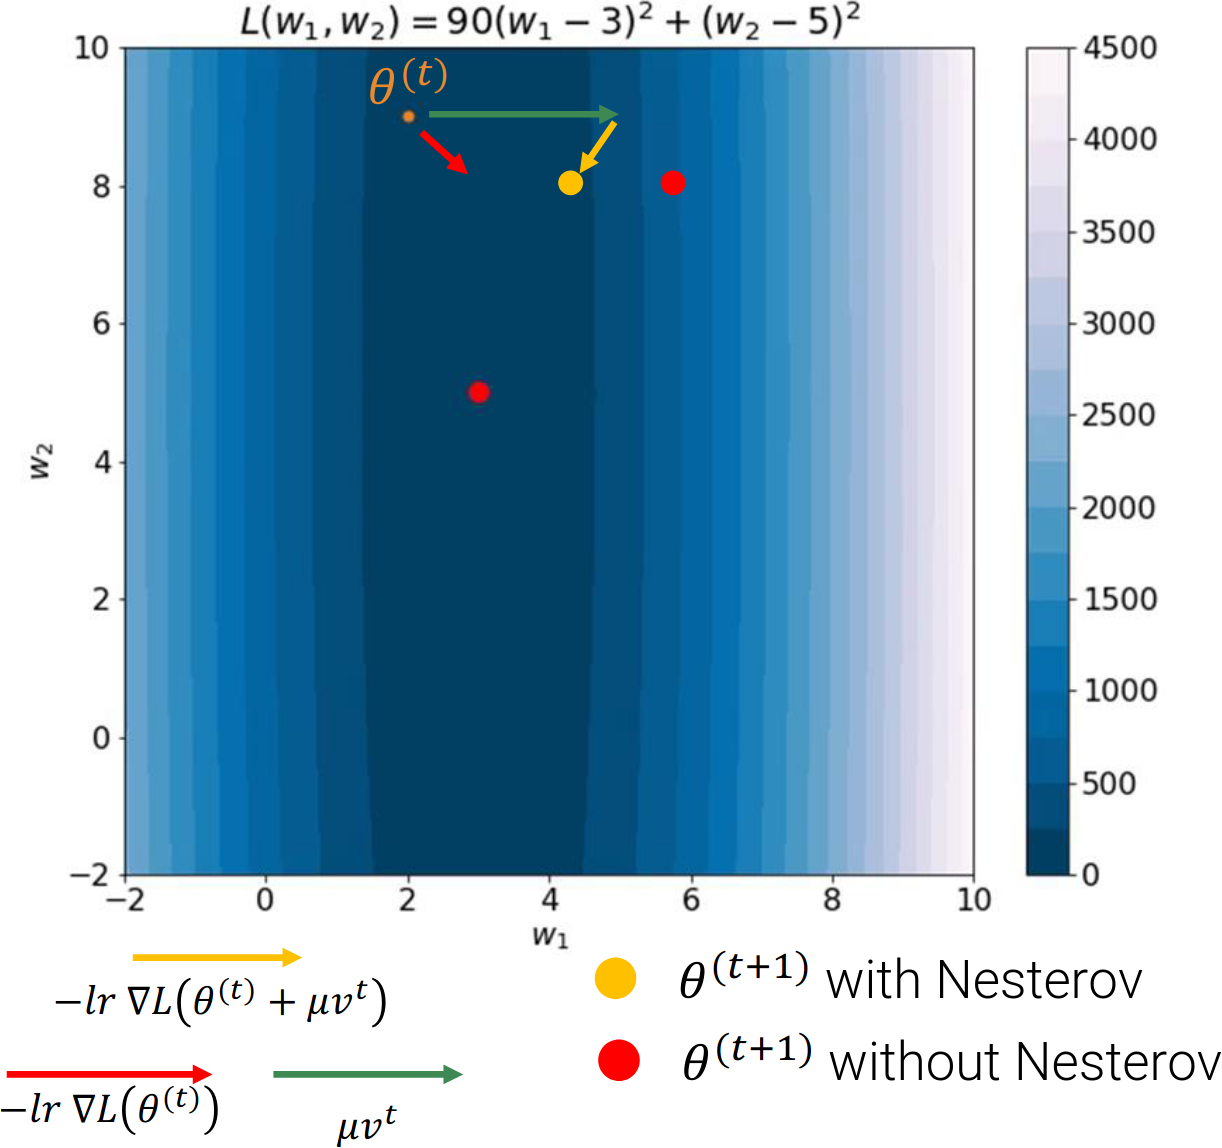
\includegraphics[width=0.35\linewidth]{./img/nesterov_momentum.png}
            \caption{Visualization of the step in Nesterov momentum}
        \end{figure}

        \begin{figure}[H]
            \centering
            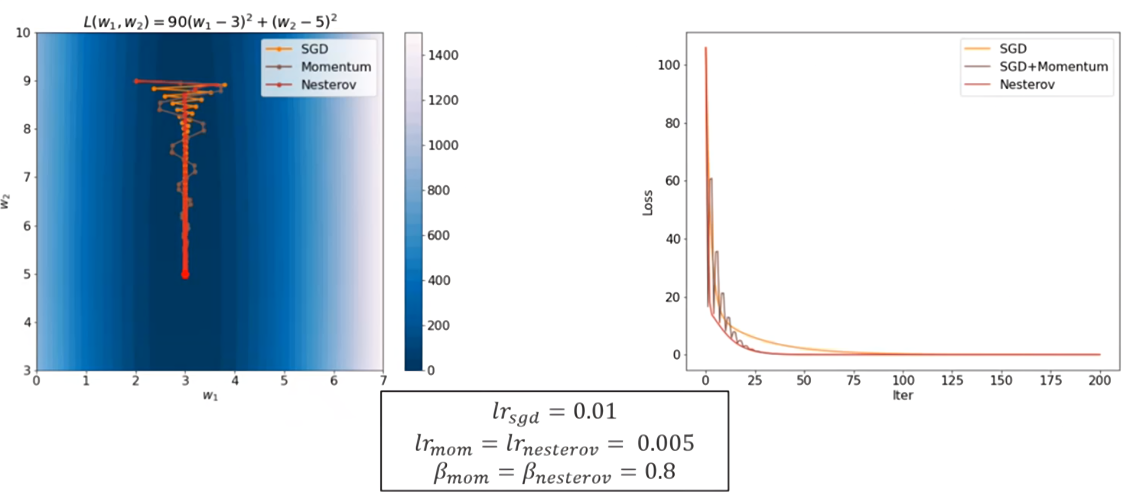
\includegraphics[width=0.75\linewidth]{./img/nesterov_comparison.png}
            \caption{Plain SGD vs standard momentum vs Nesterov momentum}
        \end{figure}
\end{description}



\section{Adaptive learning rates methods}

\begin{description}
    \item[Adaptive learning rates] \marginnote{Adaptive learning rates}
        Methods to define per-parameter adaptive learning rates.

        Ideally, assuming that the changes in the curvature of the loss are axis-aligned (e.g., in a canyon), it is reasonable to obtain a faster convergence by:
        \begin{itemize}
            \item Reducing the learning rate along the dimension where the gradient is large.
            \item Increasing the learning rate along the dimension where the gradient is small.
        \end{itemize}

        \begin{figure}[H]
            \centering
            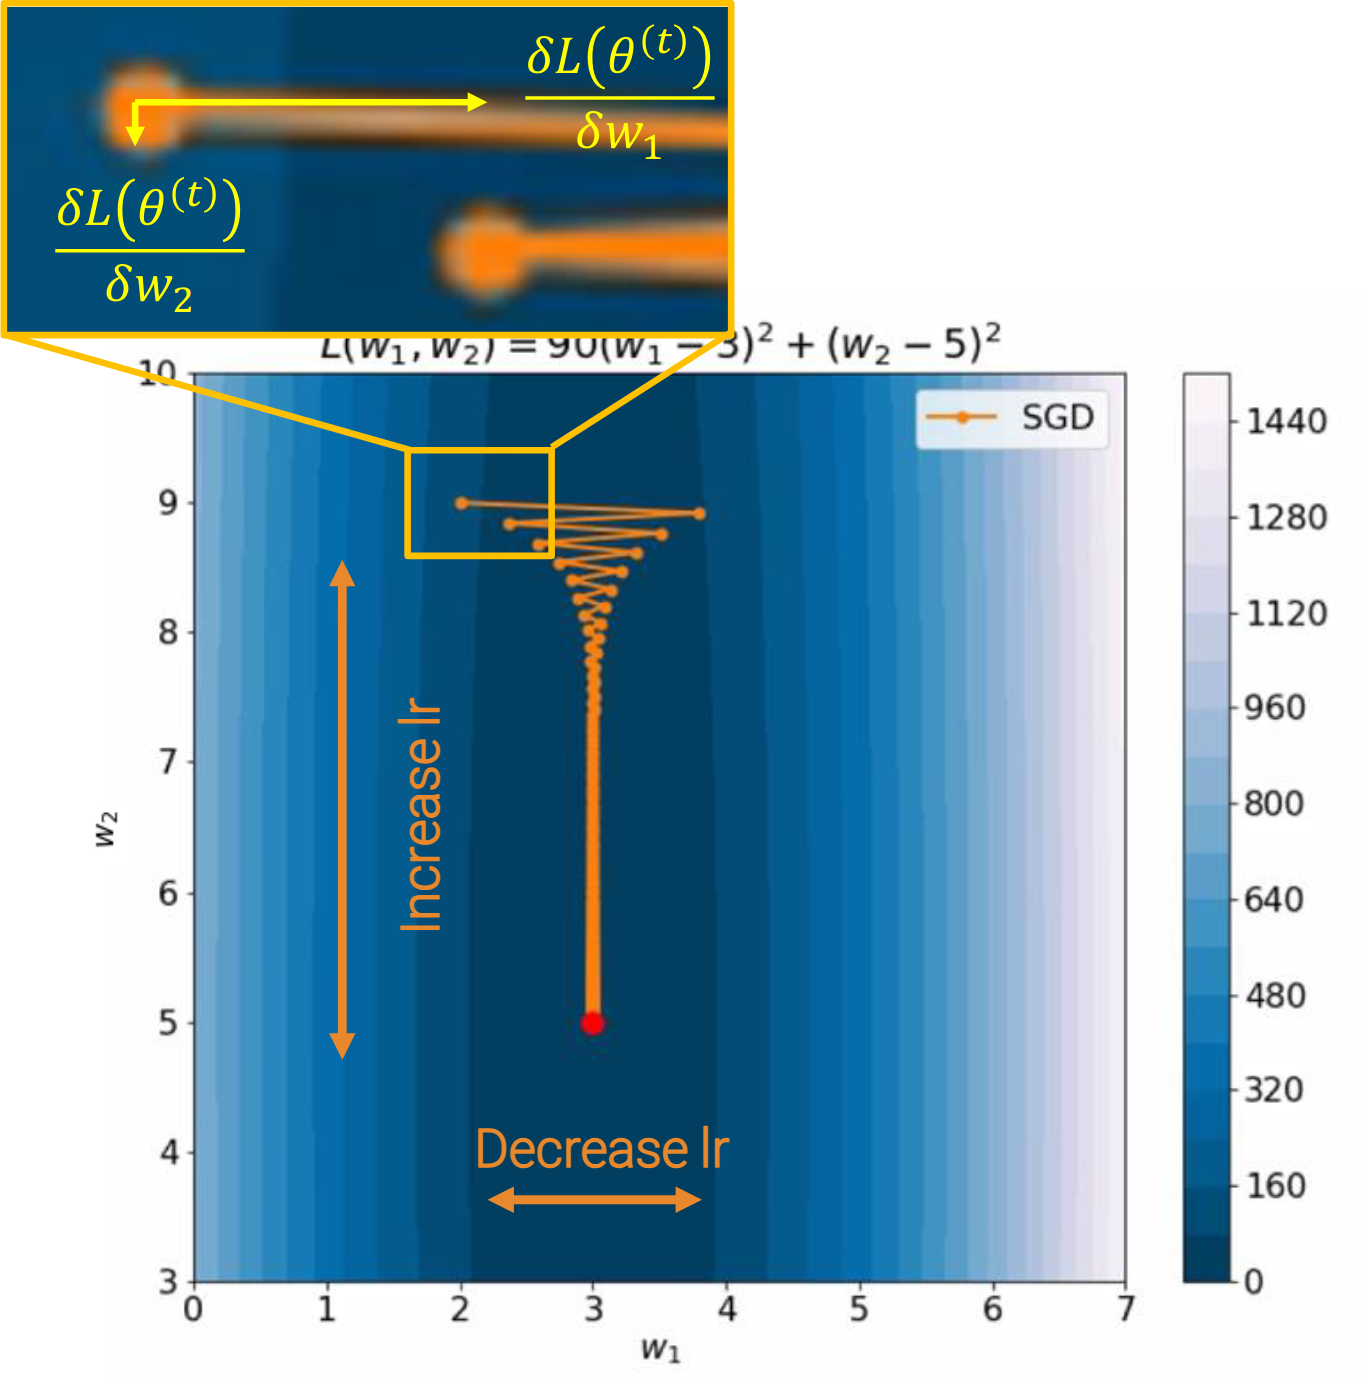
\includegraphics[width=0.35\linewidth]{./img/adaptive_lr.png}
            \caption{
                \parbox[t]{0.5\linewidth}{Loss where the $w_1$ parameter has a larger gradient, while $w_2$ has a smaller gradient}
            }
        \end{figure}

        \begin{remark}
            As the landscape of a high-dimensional loss cannot be seen, automatic methods to adjust the learning rates must be used.
        \end{remark}
\end{description}


\subsection{AdaGrad}

\begin{description}
    \item[Adaptive gradient (AdaGrad)] \marginnote{Adaptive gradient (AdaGrad)}
        Each entry of the gradient is rescaled by the inverse of the history of its squared values:
        \[
            \begin{split}
                \mathbb{R}^{N \times 1} \ni \vec{s}^{(t+1)} &= \vec{s}^{(t)} + \nabla\mathcal{L}(\vec{\theta}^{(t)}) \odot \nabla\mathcal{L}(\vec{\theta}^{(t)}) \\
                \mathbb{R}^{N \times 1} \ni \vec{\theta}^{(t+1)} &= \vec{\theta}^{(t)} - \frac{\texttt{lr}}{\sqrt{\vec{s}^{(t+1)}} + \varepsilon} \odot \nabla\mathcal{L}(\vec{\theta}^{(t)})
            \end{split}
        \]
        where:
        \begin{itemize}
            \item $\odot$ is the element-wise product.
            \item Division and square root are element-wise.
            \item $\varepsilon$ is a small constant.
        \end{itemize}

        \begin{remark}
            By how it is defined, $\vec{s}^{(t)}$ is monotonically increasing which might reduce the learning rate too early when the minimum is still far away.
        \end{remark}

        \begin{figure}[H]
            \centering
            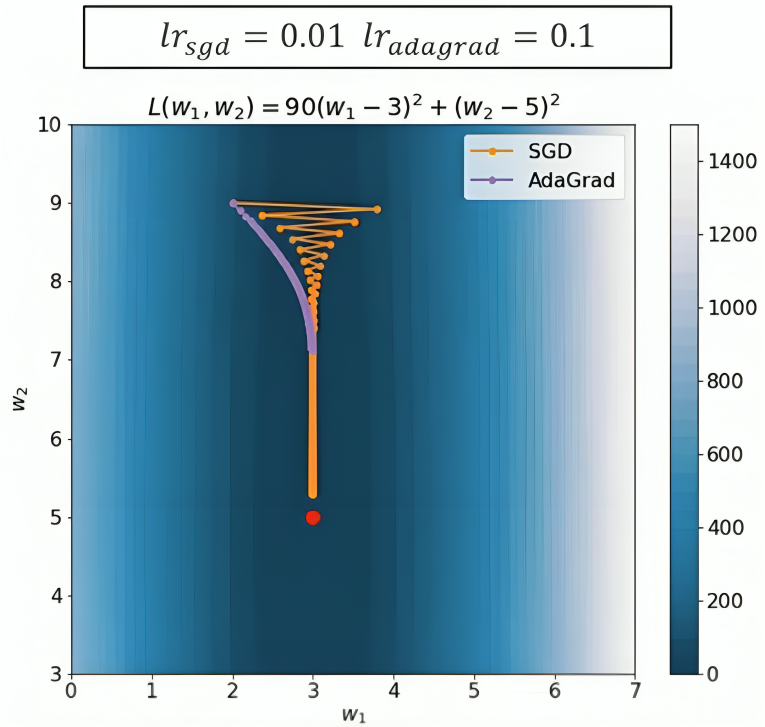
\includegraphics[width=0.4\linewidth]{./img/adagrad.png}
            \caption{
                \parbox[t]{0.45\linewidth}{SGD vs AdaGrad. AdaGrad stops before getting close to the minimum.}
            }
        \end{figure}
\end{description}


\subsection{RMSProp}

\begin{description}
    \item[RMSProp] \marginnote{RMSProp}
        Modified version of AdaGrad that down-weighs the gradient history $s^{(t)}$:
        \[
            \begin{split}
                \vec{s}^{(t+1)} &= \beta \vec{s}^{(t)} + (1-\beta) \nabla\mathcal{L}(\vec{\theta}^{(t)}) \odot \nabla\mathcal{L}(\vec{\theta}^{(t)}) \\
                \vec{\theta}^{(t+1)} &= \vec{\theta}^{(t)} - \frac{\texttt{lr}}{\sqrt{\vec{s}^{(t+1)}} + \varepsilon} \odot \nabla\mathcal{L}(\vec{\theta}^{(t)})
            \end{split}
        \]
        where $\beta \in [0, 1]$ (typically $0.9$ or higher) makes $s^{(t)}$ an exponential moving average.

        \begin{figure}[H]
            \centering
            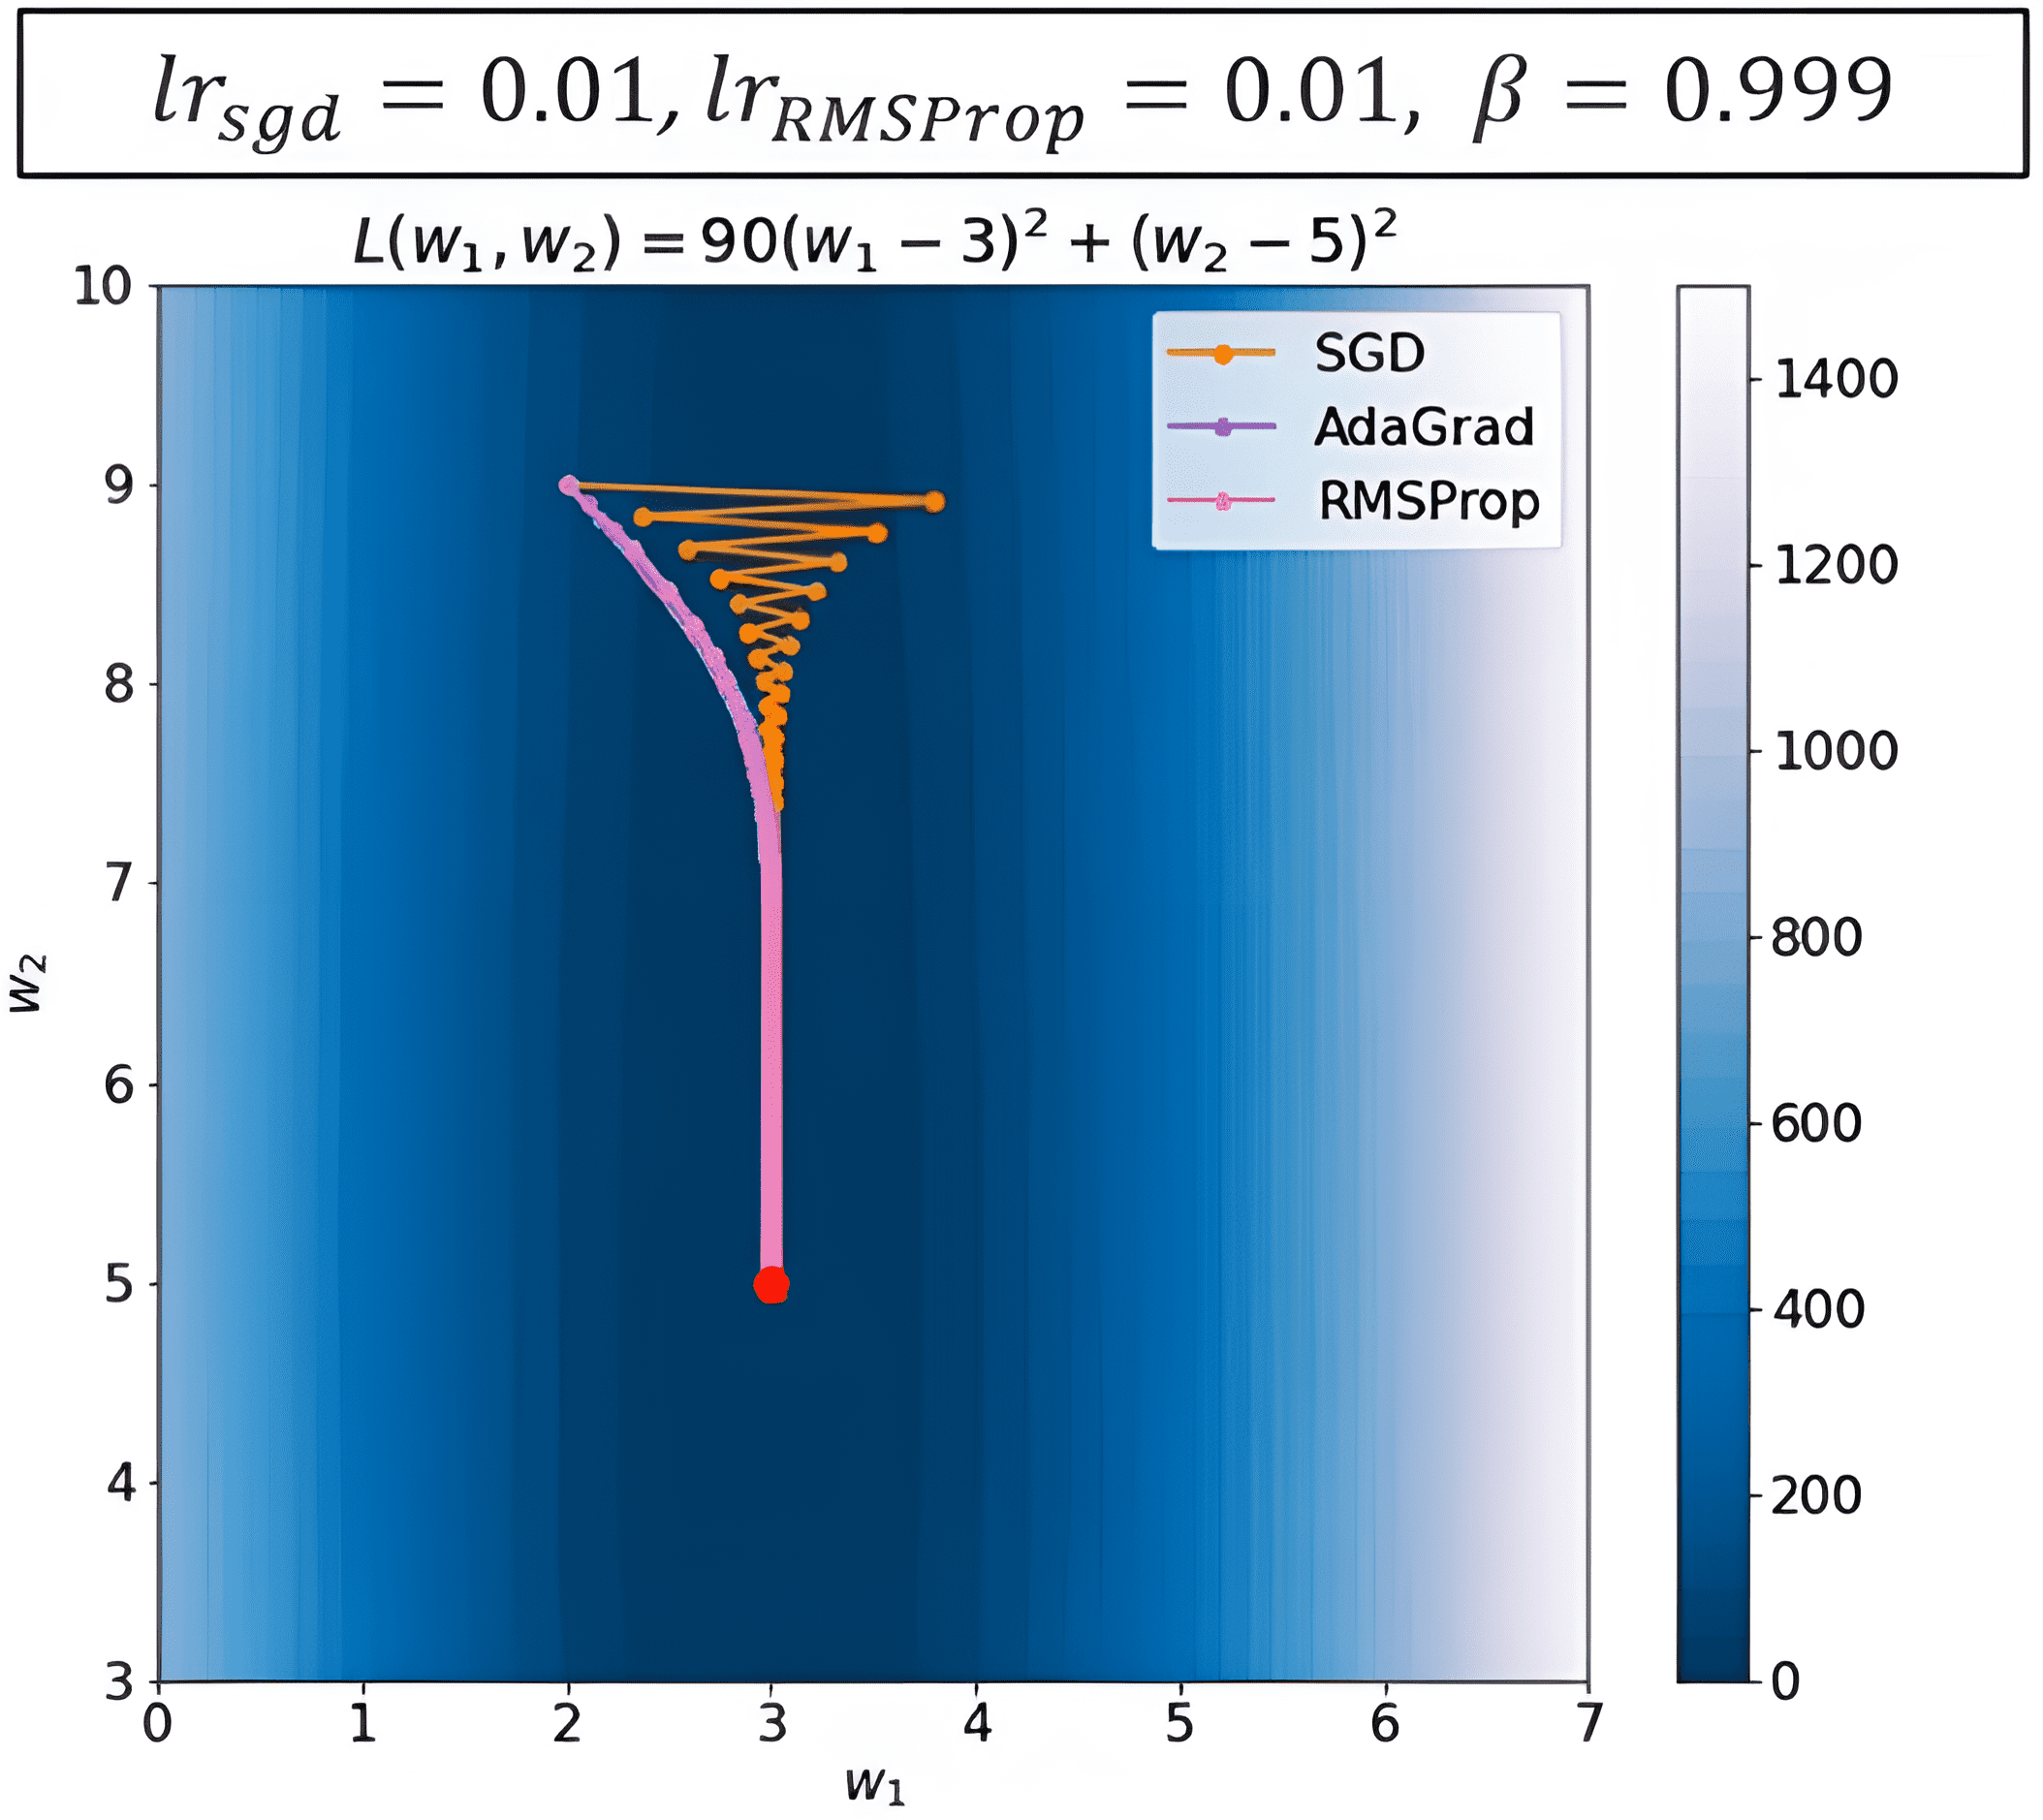
\includegraphics[width=0.4\linewidth]{./img/rmsprop.png}
            \caption{SGD vs AdaGrad vs RMSProp}
        \end{figure}
\end{description}